\chapter{Histogram clustering}

This chapter illustrates how deterministic annealing can be extended to cluster objects that do not necessarily belong to an Euclidean space. In
particular, we present here \emph{histogram clustering}, a method inspired in deterministic
annealing, to cluster objects that can be represented as histograms.

Figure~\ref{fig:image_partitioned} shows a grayscale image that has been partitioned into
patches by a cyan grid. We assume all patches to be squared and equally
sized. We want to cluster the patches by how similar they look to each
other. One could argue that there are five clusters, as there are five predominant
textures in the images. Our goal is to apply deterministic annealing
to cluster patches of an image so that patches of similar textures
are clustered together.

\begin{figure}[hbtp]
\centering
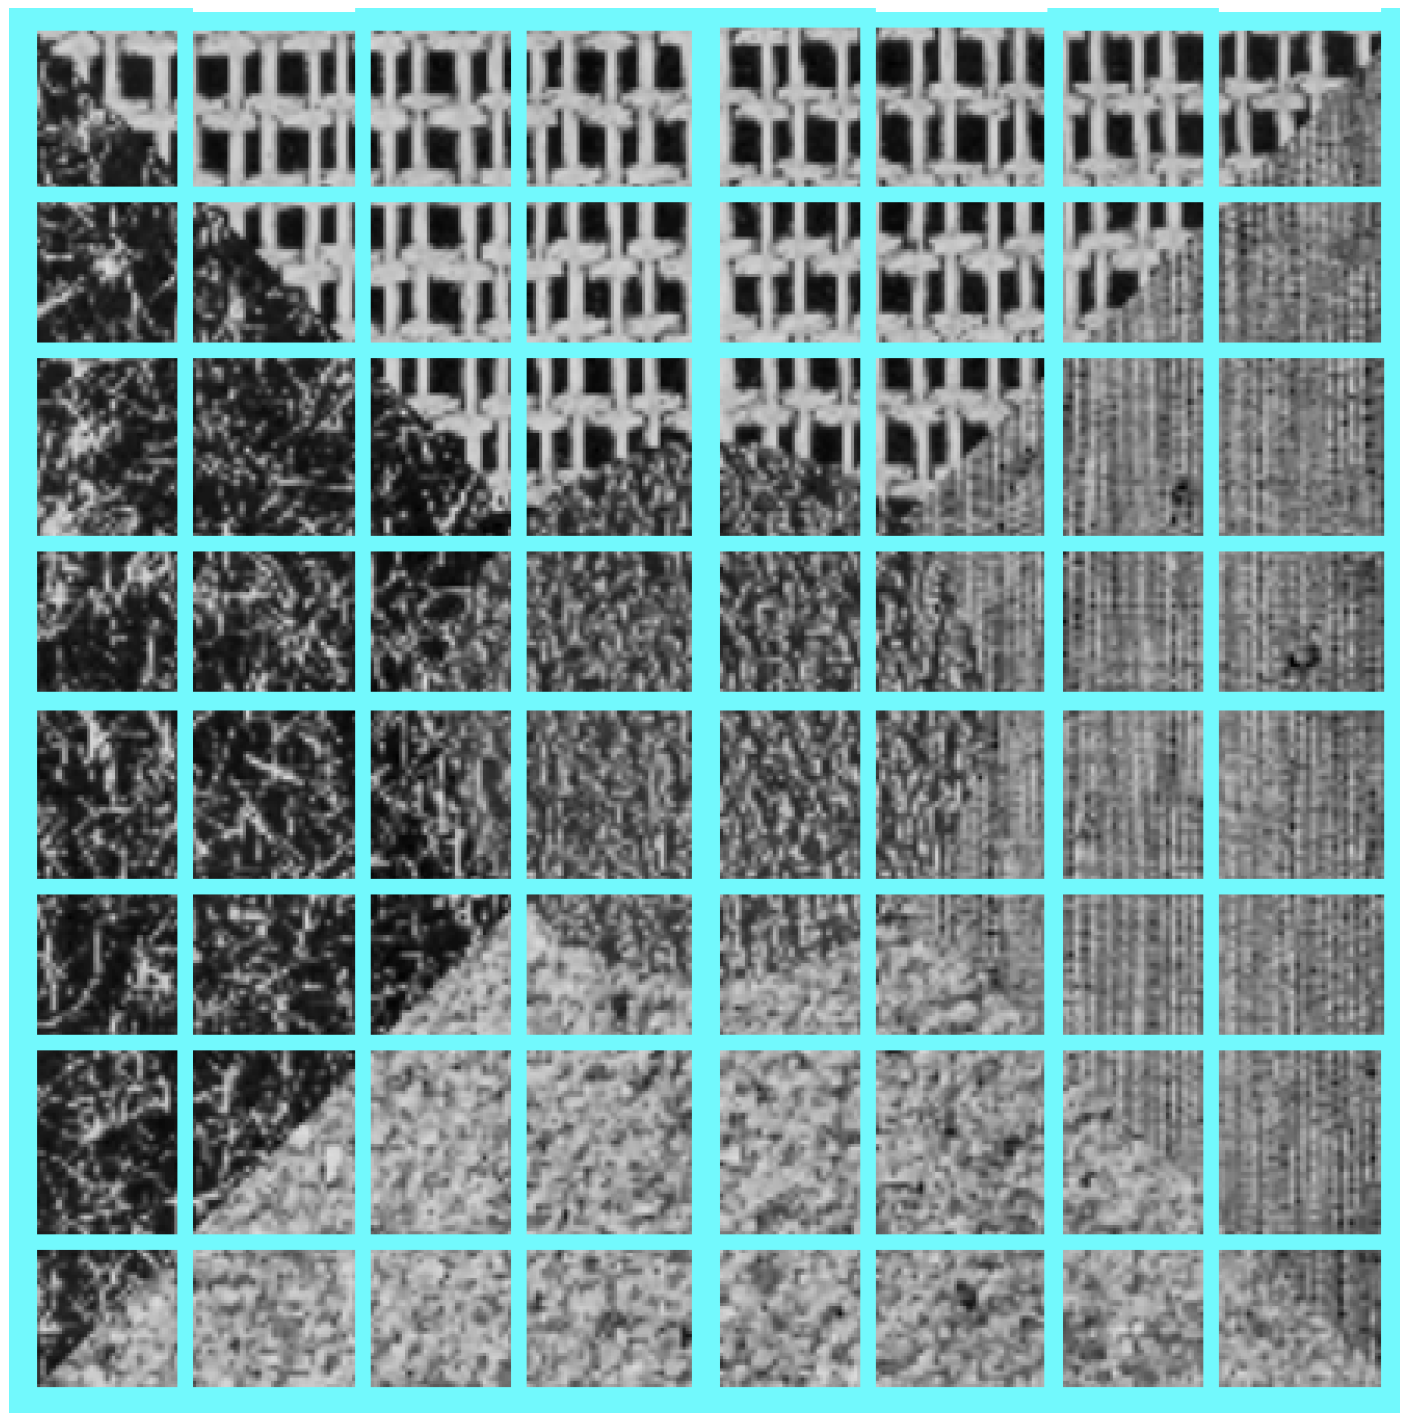
\includegraphics[width=0.4\textwidth]{\dir/five_textures}
\caption{}
\label{fig:image_partitioned}
\end{figure}

The first steps are then to define the hypothesis class and the cost function. To do this, we start by representing patches as \emph{histograms}.

\begin{definition}
A \emph{(grayscale) histogram} is a function $f : \{0, \ldots, 255\} \to [0,1]$ whose domain is the set of all possible grayscale values and such that $\sum_{b \in \{0, \ldots, 255\}} f(b) = 1$. The \emph{histogram representing a grayscale patch $x$} is the histogram $\hat{p}\left(\cdot \mid x\right)$ where $\hat{p}\left(b \mid x\right)$ counts the fraction of pixels in the patch with value $b$.
\end{definition}

We argue that two patches $x$ and $x'$ should be clustered together if their representing histograms $\hat{p}(\cdot \mid x)$ and $\hat{p}\left(\cdot \mid x'\right)$ are similar.

Histogram clustering is not restricted to clustering patches of an image.
The ideas in this chapter can be extended to other domains like clustering
documents. One can represent a document $x$ as a histogram $f : \mathcal{W} \to [0, 1]$,
where $\mathcal{W}$ denotes a set of words appearing in a text corpus. The document $x$ can be represented by the following probability mass function (pmf):

\begin{equation}
f_x(w) = \frac{\text{Number of times word $w$ occurs in $x$}}{\text{Total occurrences of all words occurring in $x$}}.
\end{equation}

The ideas in this chapter extend easily to any setting where the objects
to be clustered can be represented as such functions. This gives rise to the \emph{histogram clustering problem}.

\begin{definition}
Let $\mathfrak{X}$ be a set of \emph{objects} that are perceived only through a set $\mathcal{Y}$ of \emph{features}. Assume given a function $n : \mathfrak{X} \times \mathcal{Y} \to \mathbb{N}$ that counts $(x, y) \in \mathfrak{X} \times \mathcal{Y}$ the number $n(x,y)$ of times that feature $y$ has been observed for object $x$. The \emph{histogram} $\hat{p}\left(\cdot \mid x\right) : \mathcal{Y} \to [0, 1]$ of an object $x \in \mathfrak{X}$ is the probability mass function given by
%
\begin{equation}
\hat{p}\left(y \mid x\right) = \frac{n(x,y)}{\sum_{y \in \mathcal{Y}}n(x, y)}, \text{ for $y \in \mathcal{Y}$}.
\end{equation}
%
The problem of \emph{histogram clustering} is to cluster the objects according to histograms.
\end{definition}

Observe that for the problem of clustering image patches, the objects are
patches and the features are gray values. Also, for the problem of clustering
documents, the objects are documents and the features are words.

\section{The hypothesis class and the cost function}

For the sake of intuition, we present how to do histogram clustering in
the context of clustering patches of an image, but this presentation easily
extends to the general case.

\begin{definition}
Let $\mathcal{X}$ be the set of all images patches occurring in a given image and fix $K \in \mathbb{N}$. \emph{The hypothesis class $\mathcal{C}$ induced by $\mathcal{X}$ and $K$} is the set of all functions $c : \mathcal{X} \to \{1, \ldots, K\}$ mapping patches to cluster indices.
\end{definition}

We define a cost function that is analogous to the $K$-means cost function
from Chapter~\ref{ch:da}. This cost function is parameterized by a set $Q = \{q_1, \ldots, q_K\}$ of histograms that will act as ``centroids''. The cost function
takes then as input a function $c \in \mathcal{C}$, the set $Q$, and an image $X$ partitioned
into patches $\{x_1, \dots, x_N\}$. This function measures, for $i \leq N$, how much
$\hat{p}\left(\cdot \mid x_i\right)$ diverges from $q_{c(i)}\left(\cdot\right)$. We choose the popular Kullback-Leibler divergence
to measure this:

\begin{equation}
D_{KL}\left[\hat{p}\left(\cdot \mid x_i\right) \mid q_k\left(\cdot\right)\right] = \sum_{y \in \{0, \ldots, 255\}} \hat{p}\left(y \mid x_i\right) \log \left(\frac{\hat{p}\left(y \mid x_i\right)}{q_k\left(y\right)}\right).
\end{equation}

Based on the $K$-means cost function from Chapter~\ref{ch:da}, we now propose the following cost function.

\begin{definition}
\begin{equation}
R(c, Q, X) = \sum_{x \in \mathcal{X}} D_{KL}\left[\hat{p}\left(\cdot \mid x\right) \mid q_k\left(\cdot\right)\right].
\end{equation}
\end{definition}

\section{The Gibbs distribution}

\subsection{Efficient computation of the Gibbs distribution}

\begin{lemma}
Any Gibbs distribution $p(\cdot \mid X)$ induced by $R$ and $X$ factorizes as follows
%
\begin{equation}
p(c \mid Q, X) = \prod_{x \in X} \facprob{x}{c(x)}{Q}{X},
\end{equation}
%
where
%
\begin{equation}
\facprob{x}{k}{Q}{X} \propto \exp\left(-\frac{1}{T}D_{KL}\left[\hat{p}\left(\cdot \mid x\right) \mid q_{k}\left(\cdot \right)\right]\right), \qquad \text{for $k \leq K$}.
\end{equation}
%
\end{lemma}

\begin{proof}
The proof is very similar to the one for Theorem~\ref{thm:gibbs_factorizes} and is left as an exercise to the reader.
\end{proof}

This factorization leads to an efficient way to compute a Gibbs distribution for histogram clustering in $O(NK)$-time.

\subsection{Computing the centroids}

The centroids that maximize the entropy of a Gibbs distribution can be computed analogously to the way done in Chapter~\ref{ch:da}. Once again, we assume that the temperature hyper-parameter depends exclusively on the Gibbs distribution and not on the centroids.

\begin{exercise}
Show that the set $Q^*$ of centroids that maximize the entropy of $p(\cdot \mid Q, X)$ must satisfy the conditions:
%
\begin{equation}
q^*_k(\cdot) = \frac{\sum_{x \in X}\facprob{x}{k}{Q^*}{X}\hat{p}\left(\cdot \mid x\right)}{\sum_{x \in X} \facprob{x}{k}{Q^*}{X}}, \quad \text{for $k \leq K$,}
\end{equation}
%
\end{exercise}

Observe that this does not give a clsoed form solution to analytically compute $Q^*$. So we recur to an EM-like procedure to iteratively estimate $Q^*$.

\begin{exercise}{[Open problem!]}
Does this EM-like procedure converge to a local maximum?
\end{exercise}

\section{Histogram clustering via deterministic annealing}

Instantiating deterministic annealing for our cost function and Gibbs distribution yields Algorithm~\ref{algo:histo_cluster}

Figure~\ref{fig:phase_transitions_hc} illustrates the behavior of the centroids $Q$ when executing Algorithm~\ref{algo:histo_cluster} on the image in Figure~\ref{fig:image_partitioned}. the patches in this execution have smaller size than those shown in Figure~\ref{fig:image_partitioned}. Observe how, as the temperature decreases, the number of apparent centroids increase, following a behavior similar to the one observed in deterministic annealing.

\begin{algorithm}
\begin{algorithmic}[1]
\State Let
\State \qquad $\epsilon > 0$ be a temperature threshold,
\State \qquad $\texttt{reduce}(\cdot)$ be a function for decreasing the temperature.
\State \qquad $\texttt{close}\left(\cdot, \cdot\right)$ be a function that evaluates if two matrices are close.
\Function{DetAnn}{$\epsilon$, \texttt{reduce}, \texttt{close}}
\State $T \gets \infty$ \Comment{$\infty$ is a sufficiently large value.}
\State $Q \gets \$$ \Comment{Define arbitrary initial centroids.}
\While{$T > \epsilon$}
\Repeat
\State $Q_0 \gets Q$
\State Compute $\facprob{x}{k}{Q_0}{X}$, for $x \in X$ and $k \leq K$
\State $\displaystyle Q \gets \frac{\sum_{x \in X} \facprob{x}{k}{Q_0}{X} \hat{p}\left(\cdot \mid x\right)}{\sum_{x \in X} \facprob{x}{k}{Q_0}{X}}$, for $k \leq K$.
\Until{$\texttt{close}\left(Q, Q_0\right)$}
\State Add a small amount of noise to each centroid in $Q$.
\State $T \gets \texttt{reduce}(T)$
\EndWhile
\State \textbf{return} $Q$, $\{\facprob{x}{k}{Q}{X} \mid x \in X, k \leq K\}$
\EndFunction
\end{algorithmic}
\caption{Histogram clustering via deterministic annealing}
\label{algo:histo_cluster}
\end{algorithm}

\begin{figure}[hbtp]
\centering
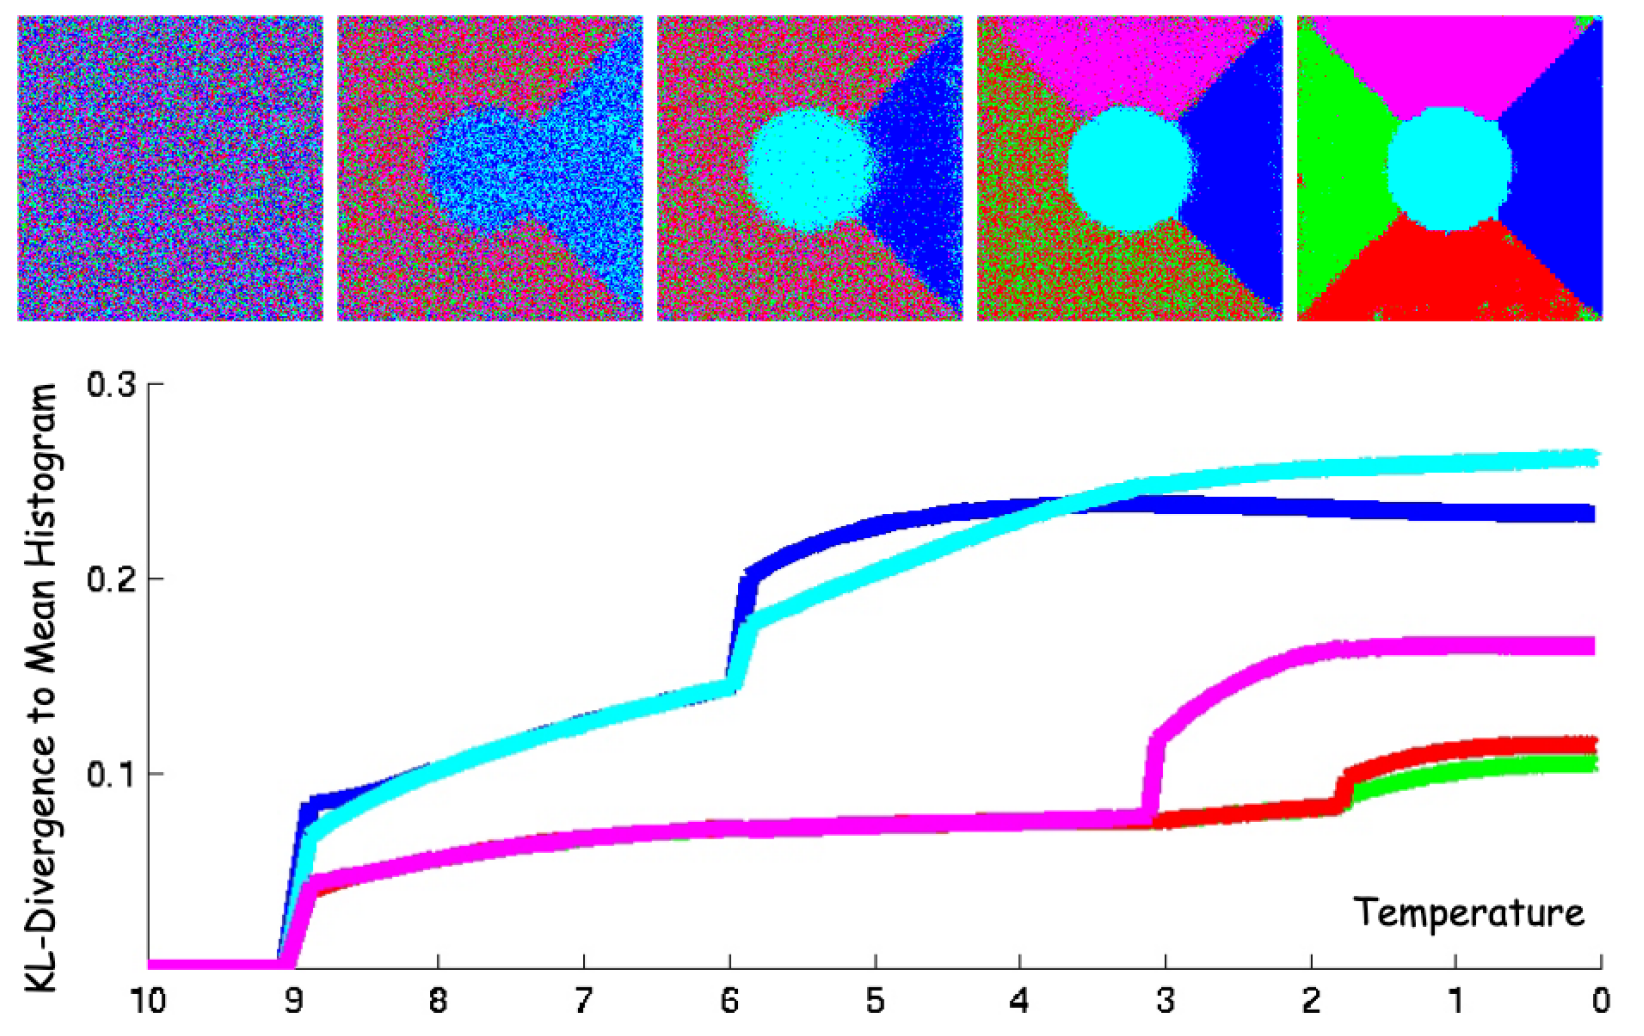
\includegraphics[width=0.8\textwidth]{\dir/phase_transitions_hc}
\caption{Histogram clustering for Figure~\ref{fig:image_partitioned}. The $x$ axis shows the temperature. The $y$ axis measures the KL-divergence between each centroid histogram and the sample mean histogram. The graphics are from Joachim Buhmann.}
\label{fig:phase_transitions_hc}
\end{figure}

\section{Histogram clustering as a probabilistic generative approach}

We can also use histogram clustering to produce a probabilistic model for
our observation. Such a model offers some benefits. We can, for example,
synthesize new observations by drawing samples from this model or define
an outlier detection system.

We define a probabilistic model for a random image. In this model, the
image is seen as a sample $(x_1, y_1), \ldots, (x_\ell, y_\ell)$ drawn from a distribution,
where $x_r$ and $y_r$ are a patch and a grayscale value, respectively. Let $\mathcal{X}$ be
the set of patches, $Q = \{q_1, \ldots, q_K\}$ be a set of centroid histograms, $\mathcal{Y}$ be
a set of grayscale values, and $c: \mathcal{X} \to \{1,\ldots, K\}$ be a function. Consider
now the following procedure.

\begin{enumerate}
\item Draw a patch $x$ from $\mathcal{X}$.
\item Draw a grayscale value $y$ from $\mathcal{Y}$ with probability $q_{c(x)}(y)$.
\end{enumerate}

This procedure induces the following pmf over $\mathcal{X} \times \mathcal{Y}$:
%
\begin{equation}
p(x, y) = p(x) q_{c(x)}(y), \text{for $(x, y) \in \mathcal{X} \times \mathcal{Y}$}.
\end{equation}
%
As $\mathcal{X}$ and $\mathcal{Y}$ are finite, one can represent $p(\cdot)$ and $q_k(\cdot)$, for $k \leq K$, as pmfs of multinomial distributions. As a result, the pmf $p(\cdot, \cdot)$ is parameterized by $p(\cdot)$, $c$, and $q_k(\cdot)$, for $k \leq K$. We denote by $\theta$ all these parameters. We can estimate these parameters via maximum-likelihood estimation (MLE).

\begin{exercise}
Start our MLE by showing that the log-likelihood $\mathcal{L}_\theta$ of a sample $\left\{|(x_1, y_1), \ldots, (x_\ell, y_\ell)|\right\}$\footnote{We use these brackets to denote a \emph{multiset}. This is necessary as $\mathcal{X}$ and $\mathcal{Y}$ are finite and we may have repeated pairs in the sample.} is:
%
\begin{equation}
\ell\sum_{x \in \mathcal{X}} \hat{p}(x) \log p(x) + \ell \sum_{x \in \mathcal{X}}\sum_{y \in \mathcal{Y}} \hat{p}\left(x, y\right) \log q_{c(x)}(y),
\end{equation}
%
where
%
\begin{equation}
\hat{p}\left(x, y\right) := \frac{n(x, y)}{\ell} = \frac{1}{\ell}\sum_{r \leq \ell} \mathbf{1}\left\{(x_r, y_r) = (x, y)\right\}, \text{and}
\end{equation}
%
\begin{equation}
\hat{p}(x) := \sum_{y \in \mathcal{Y}}\hat{p}(x, y).
\end{equation}

\textit{Hint: Show that the likelihood of the sample is}
%
\begin{equation}
\prod_{x \in \mathcal{X}}\prod_{y \in \mathcal{Y}} \left(p(x) q_{c(x)}(y)\right)^{\ell \hat{p}\left(x, y\right)}.
\end{equation}
%
\end{exercise}

\begin{exercise}
Show that
%
\begin{align}
\max_{\theta} \mathcal{L}_\theta = \max_{p(\cdot)} \ell \sum_{x \in \mathcal{X}} \hat{p}(x) \log p(x) - \\
\min_{\substack{q_1(\cdot), \ldots, q_K(\cdot)\\c}}\sum_{r \leq \ell} D_{KL}\left[\hat{p}\left(\cdot \mid x_r\right) \mid q_{c(x_r)}(\cdot)\right].
\end{align}
%
\end{exercise}

It's easy to show that the maximization problem solved by $\left(\hat{p}(x)\right)_{x \in \mathcal{X}}$. The minimization problem is equivalent to minimizing $R(c,Q, X)$ with respect to $c$ and $Q = \left\{q_k(\cdot) \mid k \leq K\right\}$, which is precisely what we do in this chapter. Hence, histogram clustering yields not only a clustering of histograms, but also a probabilistic model.